% !TeX root = ../main.tex

\chapter{结果与讨论}
\section{图表数据}
恒温槽温度:~\num{30.00}~\si{\degreeCelsius}

水$\increment h_{\si{H_2O}}=-640$~Pa~(589.5s),$\sigma_{\si{H_2O}}=\num{71.18e-3}~\si{N\cdot m^{-1}}$

毛细管常数$K'=\frac{\sigma_{\si{H_2O}}}{\increment h_{\si{H_2O}}}=\num{-1.112e-4}$

\begin{table}[h]
  \centering
  \caption{数据表格}
  \label{tab:exampletable}
  \begin{tabular}{lcccc}
    \toprule
    容量瓶编号   & 1&2&3&4  \\
    \midrule
    正丁醇用量~/~\si{mL}                  &   0.40   &   0.80   &   1.20   &   1.60   \\
    溶液浓度~$c$~/~\si{mol\cdot L^{-3}}   &    \num{4.37e-2} & \num{8.74e-2} & \num{1.31e-1} & \num{1.75e-1} \\
    最大压差读数~$\increment h$~/~\si{Pa} & -556~(244.3s)  &   -498~(54.0s)  &  -458~(105.7s)  & -425~(121.6s)     \\
    正丁醇水溶液的$\sigma$                & \num{6.18e-2} & \num{5.54e-2} & \num{5.09e-2} & \num{4.73e-2}      \\
      正丁醇水溶液的$\dif \sigma / \dif c$  & \num{-2.01e-1}  &	\num{-1.13e-1}  &	\num{-9.19e-2}  &	\num{-8.04e-2}       \\
    正丁醇水溶液的$\Gamma$                & \num{3.48E-06}  &	\num{3.93E-06}  &	\num{4.78E-06}  &	\num{5.58E-06}       \\
    正丁醇水溶液的$c/\Gamma$              & \num{1.26e4} &	\num{2.22e4} &	\num{2.74e4} &	\num{3.13e4}       \\
    \bottomrule
  \end{tabular}
\end{table}
~~~~~~~~~(续表)
\begin{table*}[h]
  \centering
  \begin{tabular}{lccc}
    \toprule
    容量瓶编号   & 5&6&7  \\
    \midrule
    正丁醇用量~/~\si{mL}                  &   2.00   &   2.40   &   2.80       \\
    溶液浓度~$c$~/~\si{mol\cdot L^{-3}}  &  \num{2.19e-1} & \num{2.62e-1} & \num{3.06e-1}    \\
    最大压差读数~$\increment h$~/~\si{Pa} & -396~(65.6s) &  -379~(106.7s) & -361~(109.1s)   \\
    正丁醇水溶液的$\sigma$                & \num{4.405e-2} & \num{4.22e-2} & \num{4.01e-2}       \\
    正丁醇水溶液的$\dif \sigma / \dif c$  &  \num{-5.77e-2}	& \num{-3.75e-2}	& \num{-6.62e-2}      \\
    正丁醇水溶液的$\Gamma$                & \num{5.01E-06}  &	\num{3.90E-06}  &	\num{8.04E-06}        \\
    正丁醇水溶液的$c/\Gamma$              & \num{4.37e4} &	\num{6.72e4} &	\num{3.80e4}       \\
    \bottomrule
  \end{tabular}
\end{table*}

作图如图\ref{fig1},图\ref{fig2}所示.

\section{结果讨论}

由图\ref{fig1},图\ref{fig2}可知\\
$\sigma = -78.242c^5 + 70.436c^4 - 24.125c^3 + 4.1029c^2 - 0.443c + 0.0751,~R^2 = 1\\
\dif \sigma / \dif c=-391.21c^4 + 281.744c^3 - 72.375c^2 + 8.2058c - 0.443\\
\Gamma_{\infty}=149182\\
S_0=\frac{1}{\Gamma_{\infty}\widetilde{N} }=\num{1.1131221e-29}~\si{m^2}
$



\begin{figure}[h]
  \centering
  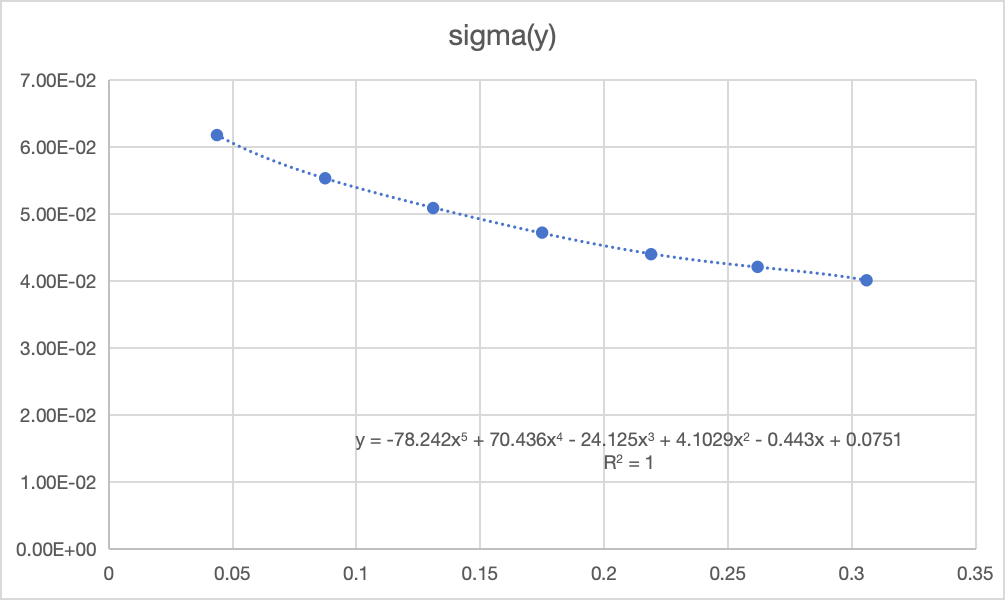
\includegraphics[width=1\textwidth]{fig1.png}
  \caption{$\sigma -c$图}
  \label{fig1}
\end{figure}

\begin{figure}[h]
  \centering
  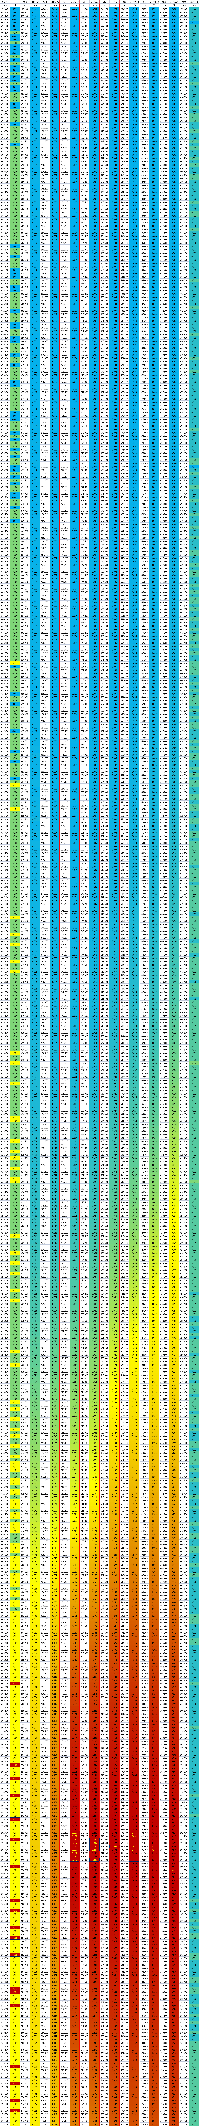
\includegraphics[width=1\textwidth]{fig2.png}
  \caption{$c/\Gamma -c$图}
  \label{fig2}
\end{figure}



\section{误差来源}
误差与仪器气密性、拟合精度等有关.

\section{体会认识}
了解表面张力的性质、表面能的意义以及表面张力和吸附的关系;
掌握了一种测定表面张力的方法—最大气泡法.
